\documentclass{standalone}
\usepackage{tikz}
\usepackage{amsmath,amsfonts,amssymb,xcolor}
\usepackage{enumitem,graphicx}
\newcommand{\Cross}{$\mathbin{\tikz [x=1.4ex,y=1.4ex,line width=.2ex, red] \draw (0,0) -- (1,1) (0,1) -- (1,0);}$}%
\newcommand{\Checkmark}{$\color{green}\checkmark$}
\begin{document}
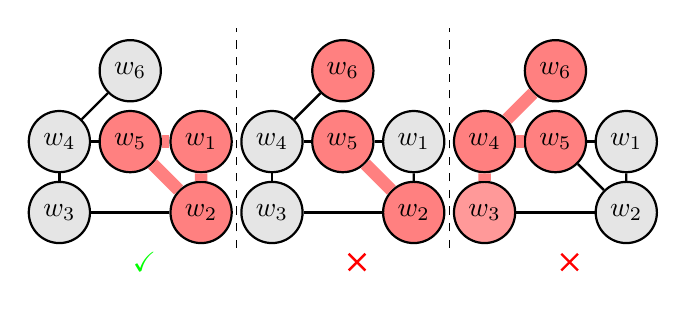
\begin{tikzpicture}[scale=.9,auto=left,every node/.style={draw,circle,thick,fill=black!10}]
\node (n16) at (1,9)  {${w}_6$};
\node (n14) at (0,8)  {${w}_4$};
\node[fill=red!50] (n15) at (1,8)  {${w}_5$};
\node[fill=red!50] (n11) at (2,8)  {${w}_1$};
\node[fill=red!50] (n12) at (2,7)  {$w_2$};
\node (n13) at (0,7)  {$w_3$};
%-------------
\node[fill=red!50]  (n26) at (4,9)  {$w_6$};
\node (n24) at (3,8)  {$w_4$};
\node[fill=red!50]  (n25) at (4,8)  {$w_5$};
\node (n21) at (5,8)  {$w_1$};
\node[fill=red!50]  (n22) at (5,7)  {$w_2$};
\node (n23) at (3,7)  {$w_3$};
%------------
\node[fill=red!50]  (n36) at (7,9)  {$w_6$};
\node[fill=red!50]  (n34) at (6,8)  {$w_4$};
\node[fill=red!50]  (n35) at (7,8)  {$w_5$};
\node (n31) at (8,8)  {$w_1$};
\node (n32) at (8,7)  {$w_2$};
\node[fill=red!40]  (n33) at (6,7)  {$w_3$};
\foreach \from/\to in {n16/n14,n14/n15,n12/n13,n13/n14,
n26/n24,n24/n25,n25/n21,n21/n22,n22/n23,n23/n24,
n35/n31,n31/n32,n32/n35,n32/n33}
\draw[line width=0.3mm] (\from) -- (\to);
\foreach \from/\to in {n15/n11,n11/n12,n12/n15}
\draw[line width=1.6mm, red!50] (\from) -- (\to);
\foreach \from/\to in {n22/n25}
\draw[line width=1.6mm, red!50] (\from) -- (\to);
\foreach \from/\to in {n36/n34,n34/n35,n33/n34}
\draw[line width=1.6mm, red!50] (\from) -- (\to);
\draw[dashed] (2.5,6.5) -- (2.5,9.6);
\draw[dashed] (5.5,6.5) -- (5.5,9.6);

\node[draw=white,fill=white] at (1.2, 6.3)  {\Checkmark};
\node[draw=white,fill=white] at (4.2, 6.3)  {\Cross};
\node[draw=white,fill=white] at (7.2, 6.3)  {\Cross};
\end{tikzpicture}
\end{document}
% \caption{A toy example of Weighted Graph Model}
